\chapter{Introduction}


\vspace{2mm}

\section{Motivation}
\textbf{Author: Sztavinovszki}

In almost every robotics application nowadays you need some kind of communication. Wether it is a robot communicating
its data to a home-base, or two robots sharing data with one another. Over the past years communication has drastically
improved with new protocols and technology, such as Bluetooth Low energy. On the other hand there are still people, that
don't use any of the communication technologies described before, because most of the established frameworks are seem to
complex or have too many requirements regarding performance.

\section{Goal}
\textbf{Author: Sztavinovszki}

This diploma thesis will take explore how to write a communication framework using new technologies, such as BLE with TCP
and UDP.
At the end of the project the framework should be useable for sending data between two KIPR Wombat-Controllers. It should be capable
to send well structured data, e.g. a JSON-file, as well as streaming data, e.g. a series of pictures, between the robots.

\section{History}

\section{Project Management}
\textbf{Author: Sztavinovszki}

\section{Outline}
%\section{Section}
%More text. \lipsum[1] See Figure~\ref{pic:example}.

%\begin{figure}[h]
%	\centering
%	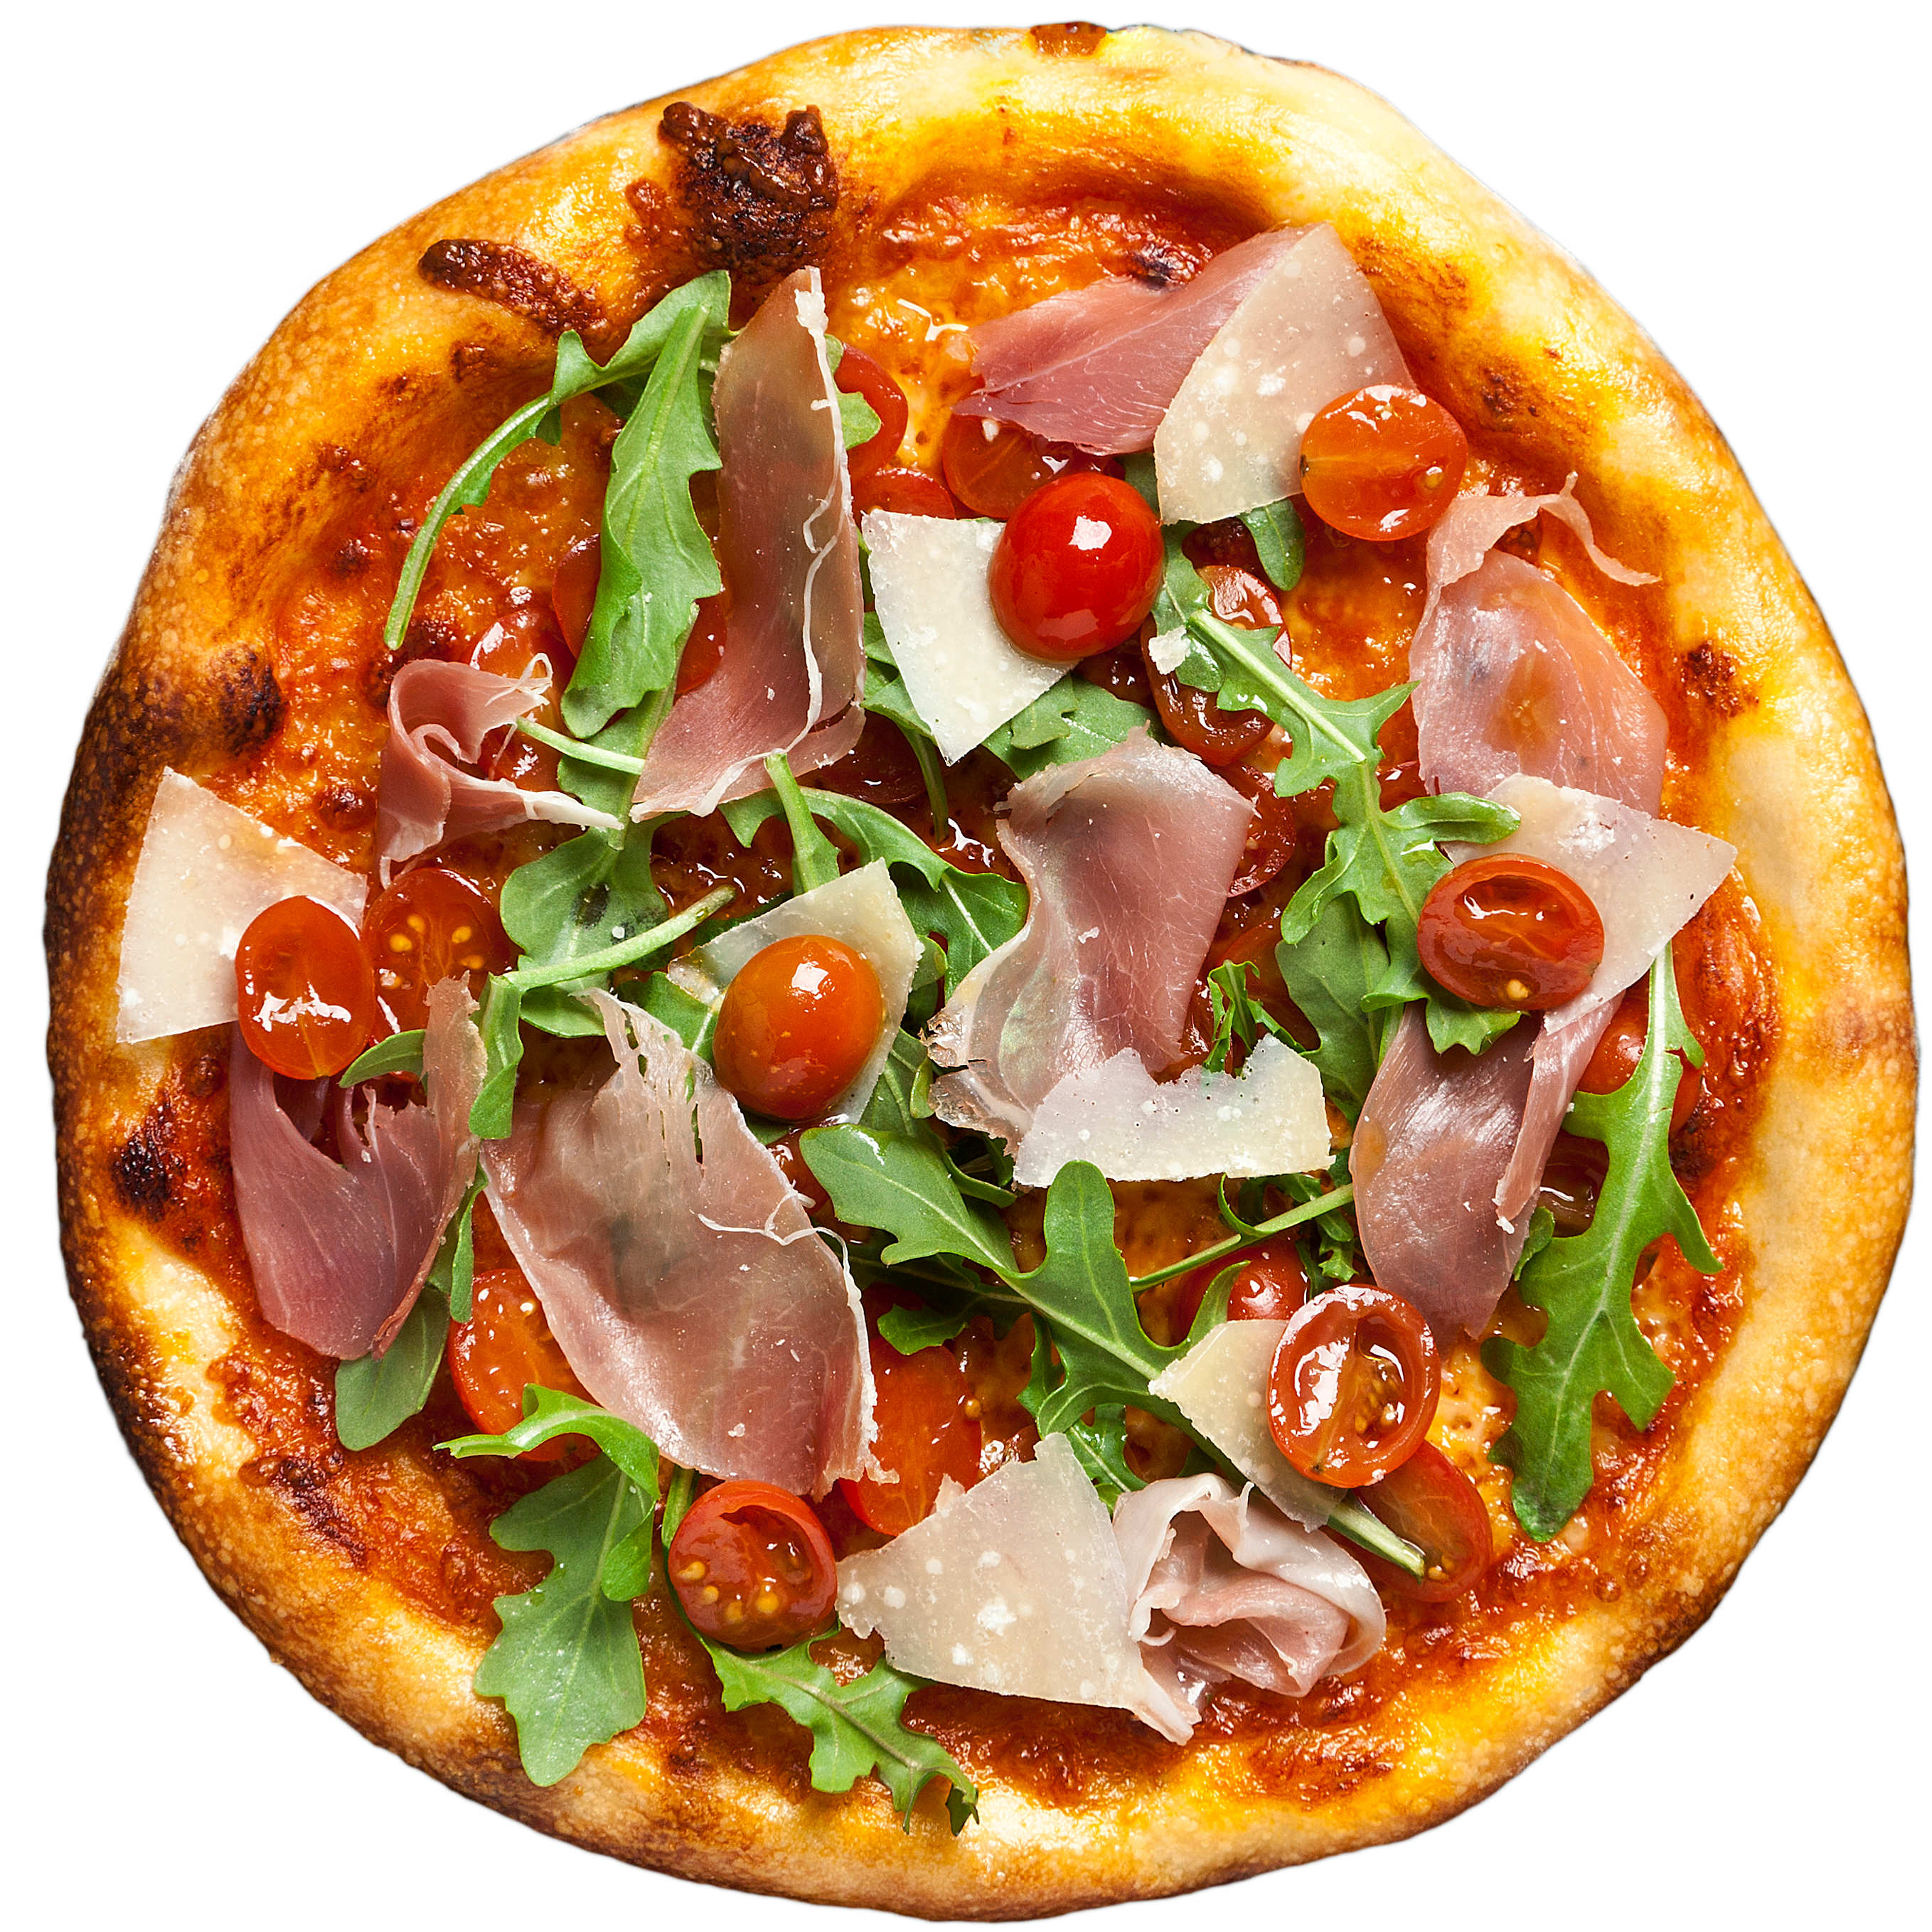
\includegraphics[width=2.5in]{img/example.png}
%	\caption{Picture description.}
%	\label{pic:example}
%\end{figure}

%\subsection{Subsection}
%\lipsum[1]

%\subsection{Subsection}
%\lipsum[1] See Table~\ref{tab:example}.

%\begin{center}
%	\begin{tabular}{| l | l | l |}
%		\hline
%		\bfseries Header 1 & \bfseries Header 2 & \bfseries Header 2 \\
%		\hline
%		Text & text & text \\
%		\hline
%		Text & text & text  \\
%		\hline
%		Text & text & text  \\
%		\hline
%	\end{tabular}
%	\label{tab:example}
%\end{center}

%\lipsum[1] Some references can be found at \footcite{robo4you} or at \footcite{Hope_Learning_TensorFlow}.
%

\filbreak
